\section{Experiments}
\label{Sec:Experiments}

% This section evaluate Cerberus by answering several key questions.
% \begin{itemize}
%         \item \textbf{Q1}: will Cerberus improve application performance
%                 by utilizing burst buffer nodes?
%         \item \textbf{Q2}: Will job demand on burst buffer affect Cerberus?
%                 Why bother to divide the job execution into 3 phases?
%         \item \textbf{Q3}: Can dynamic programming based optimization
%                 help Cerberus further
% improve application performance?
% \end{itemize}
% Our newly developed event-driven simulator, BBSim, is used to simulating
% the Trinity system described later.

%==============XY===================
This section evaluates Cerberus by answering three key questions.
\begin{itemize}
        \item \textbf{Q1}: Does the use of burst buffer 
        improve both system-level and job-level performance?\NOTE{keep unchanged}
        \item \textbf{Q2}: What is the benefit of using 
        fine-grained three-phase scheduling?
        \item \textbf{Q3}: What is the performance gain achieved 
        by Cerberus optimization based scheduling?
\end{itemize}

% metric

% We select two evaluation metrics, job's \textit{response time} and 
% \textit{system throughput}, when evaluating our design.
% Response time is the time duration from job submission to its fully completion,
% which is the major concern from user's perspective.
% On the other hands, system throughput, defined as the number of jobs finished in
% a fixed time period (500 seconds), measures the performance of computing system.

%==============XY===================
We select three evaluation metrics, \textit{job response time}, \textit{job waiting time} and \textit{system throughput}.
Job response time is the time duration between the job submission and the job completion. Job waiting time is the total time that a job waits in each queue.
System throughput is defined as the number of jobs completed in a fixed time period (500 seconds).

%
%\subsection{Experimental Settings}
%% % system
%% We consider simulating the full Trinity super computer\cite{TrinitySystem}.
%% The number of compute nodes on Trinity is about 18,936,
%% e.g. 9,436 Intel Haswell nodes
%% and at least 9500 Intel Xeon Phi nodes.
%% There are 16 cores on each processor, thus totally 302,976 cores.
%% In the following experiments, we compare two identical system except that
%% IO nodes are replaced by the same number of burst buffer nodes.
%% Eventually Trinity plans to delivery up to 576 burst buffer nodes of 3.7 PB,
%% consisted of Trinity IO nodes with PCIe SSD card.
%% They are globally accessible as intermediate storage and distributed among cabinets.
%% Sequential read/write speed of burst buffer nodes is 8.0 GBps.
%% Bandwidth between CPU node and non-burst-buffer IO node is set to 2.5 GBps.
%
%
%We simulate a burst-buffer-enabled system as shown in Figure~\ref{Fig:BBArchitecture}.
%This system architecture is inspired by Trinity~\cite{TrinitySystem}, 
%the next generation supercomputer in Los Alamos National Laboratory.
%The parameters used in our simulation are taken from the 
%Trinity/NERSC-8 Use Case Scenarios technical report\cite{BBUseCase}.
%The simulated system consists of 18,936 compute nodes,
%e.g., 9,436 Intel Haswell nodes and 9,500 Intel Xeon Phi nodes.
%There are 576 burst buffer nodes with an aggregated 3.7 PB storage, which are globally accessible as the intermediate storage.
%The sequential read/write speed of burst buffer nodes is 8.0 GBps.
%The bandwidth between a CPU node and an IO node is set to 2.5 GBps.
%
%\begin{figure}[htp]
%        \centering
%        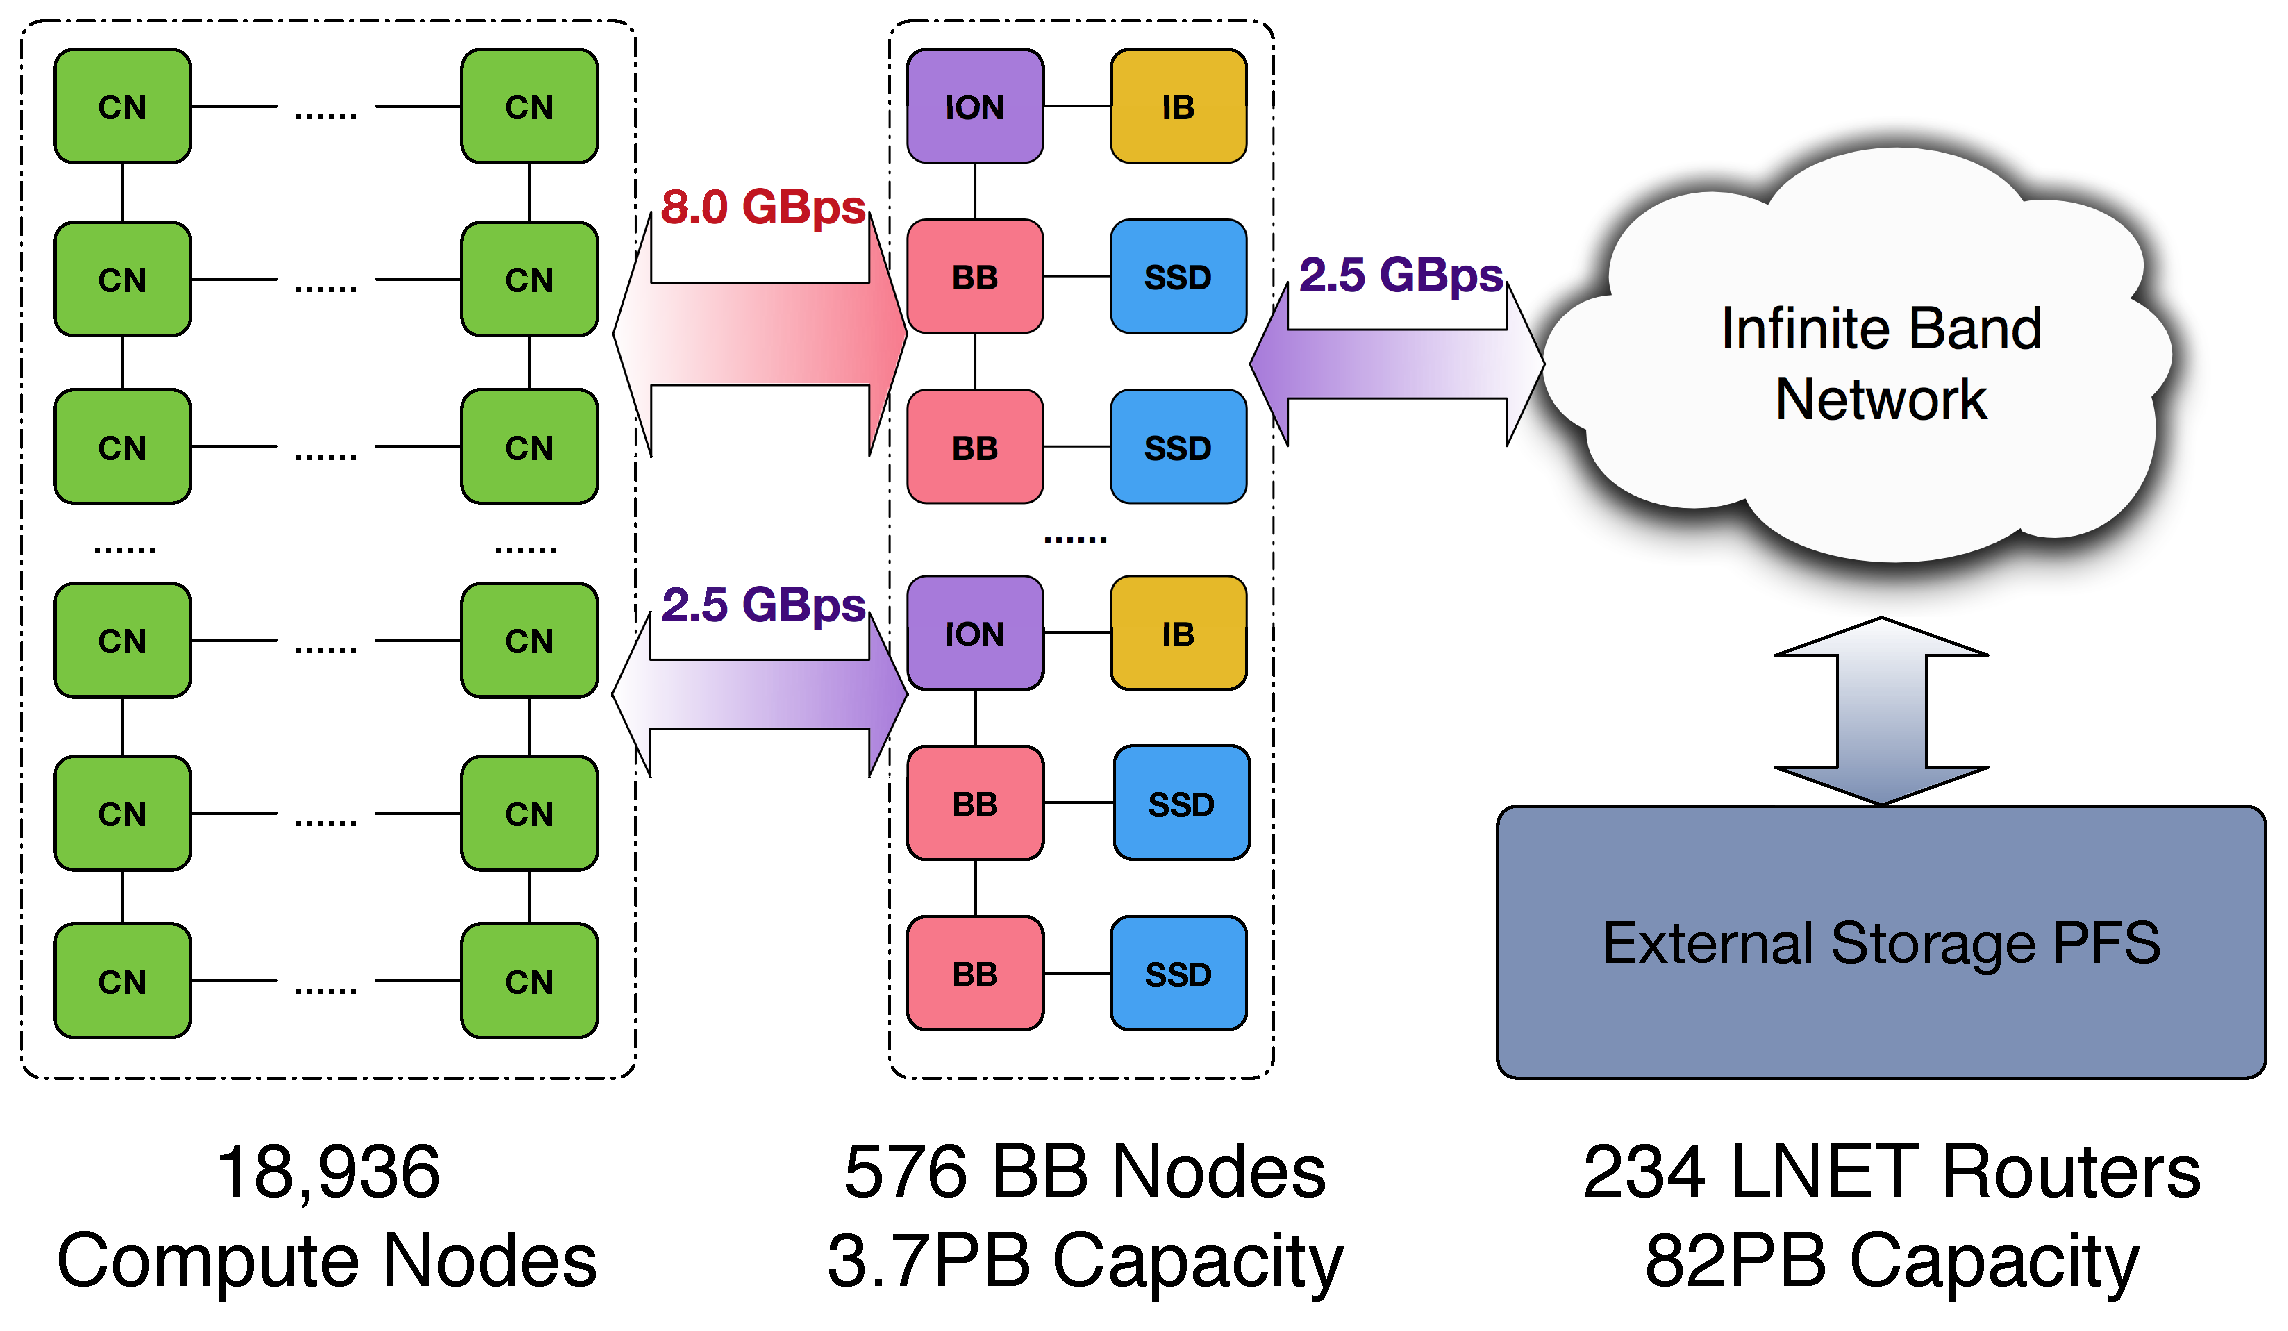
\includegraphics[width=3.5in]{BBArchitecturewithBandwidth}
%        \caption{Our simulated burst buffer enabled HPC system inspired by Trinity at LANL\TODO{remove the blue SSD nodes in Fig}}
%        \label{Fig:BBArchitecture}
%\end{figure}
%
%% % trace
%% Job trace is from ANL's Blue Gene Intrepid system,
%% containing totally 68,936 jobs run during January to September 2009\cite{JobTrace}.
%% We extract two critical fields from this jobs trace: running time and
%% number of cores user requested.
%% In this section we take a window of 1,185 jobs and report their scheduling results.
%% We patched 3 fields to each job's log entry: the amount of input data $data\_in$,
%% the total amount of written data for checkpointings $data\_run$
%% and the amount of output data $data\_out$.
%% We assume $data\_run$ and $data\_out$ follows uniform distribution with
%% lower boundary of 1 TiB and upper boundary of 60 TiB;
%% $data\_in$ follows uniform distribution between 1 GiB and 30 Gib.
%% The patches 3 fields may or may not be used in scheduling,
%% depends on both the model of the jobs and the experiment scenario.
%
%
%Since Trinity is not available to use at present, there is no Trinity job log available for our study.
%We use the job log collected from ANL's Blue Gene Intrepid system. The log contains 68,936 jobs
%submitted to the system from January to September 2009~\cite{Tang:IPDPS:2010}.
%We patched 3 fields to each job's log entry: the amount of input data $data\_in$,
%the total amount of written data for checkpointings $data\_run$
%and the amount of output data $data\_out$.
%We assume $data\_run$ and $data\_out$ follows the uniform distribution with a
%lower bound of 1 TB and a upper bound of 60 TB;
%$data\_in$ follows the uniform distribution between 1 GB and 30 GB~\cite{Liu:MSST:2012}.
%
% \subsection{BB-Enabled System v.s. IO-Node-Only System}
\subsection{Utilizing Burst Buffer v.s. Direct IO}
\label{Sec:Sim:DirectIOvsBB}
% In this section, we demonstrate that by utilizing burst buffer nodes,
% job scheduler could improve the performance of both applications and system.
% We compare two systems:
% \begin{itemize}
%         \item \textbf{1-Phase IO}: system without burst buffer nodes
%                 scheduled by FCFS policy
%         \item \textbf{Cerberus}: system with burst buffer 
%                 scheduled by our proposed Cerberus
% \end{itemize}


%=============XY==============

PFS is mounted by all the compute nodes in the Trinity architecture, thus applications have the
option to bypass the burst buffer and to use the file system directly for their IO operations.
We refer this scenario as \textit{Direct IO}. Apparently, the performance of \textit{Direct IO}
is limited by the low bandwidth of the IO nodes. However, applications will be exempted from
waiting in the stage-in and stage-out phases in the case of \textit{Direct IO} rather than utilizing the burst buffer.
In this section, we compare the performance of applications utilizing the burst buffer
against \textit{Direct IO}.
Based on the comparison, we answer question \textbf{Q1}: by utilizing burst buffer nodes,
both the job-level and system-level performance can be significantly improved.


% Figure~\ref{Fig:DirectIOvsBBResponse} compares CDF of the response time of 1185 jobs.
% When scheduler can allocate burst buffer to jobs,
% response time is bounded by 376,443.12 seconds.
% However, the worst case in system without burst buffer
% (Direct IO) is catastrophical.
% There are jobs that takes 889,239.20 seconds to finish,
% which is 2.36 times slow as the most non-responsive job
% in system equipped with burst buffer.
% In average case, \textit{nearly 99\% of the jobs scheduled by Cerberus
% response faster than Direct batch scheduler on non-BB system.}
% The improvement mainly comes from the difference of IO operation efficiency between
% traditional IO nodes and burst buffer nodes.

%=============XY==============
Figure~\ref{Fig:DirectIOvsBBResponse} compares CDF of the job response
time on the burst-buffer-enabled system and the traditional system (Direct IO).
For the burst-buffer-enabled system, the job response time is bounded by 376,443.12 seconds.
However, the worst case of Direct IO is catastrophic, i.e., a job takes 889,239.20 seconds to finish, which is 2.36 times slower than the slowest non-responsive job
in the burst-buffer-enabled system.
In average, \textit{nearly 99\%} of the jobs scheduled on the burst-buffer-enabled system
response faster than the traditional system without burst buffer, since the burst buffer can mitigate the IO gap between IO nodes and compute nodes.


% Figure~\ref{Fig:DirectIOvsBBWait} reveals the total waiting time for both cases.
% Notice that system without burst buffer only request compute nodes.
% In this case, waiting time is the duration from its submission
% to actual starting running.
% The difference of worst case waiting time is drastic.
% Without burst buffer nodes, job's wait duration in worst case is 3.02 times
% slow as the worst one on systems with burst buffer;
% the upper bound of waiting duration for burst buffer systems is about 285,254 seconds.
% Because of burst buffer's better ability to
% absorb checkpoint operations and data moving in/out,
% the execution pipeline of job series is significantly speed up.
% Statistically, \textit{more than 80\% jobs waited less time, thus response faster,
% if they can access burst buffer.}

%=============XY==============
Figure~\ref{Fig:DirectIOvsBBWait} reveals the aggregated job waiting time.
Note that in the case of Direct IO, jobs only request compute nodes.
Thus, the waiting time is the duration between the job submission and the job starting time.
The difference about the worst case waiting time in the both systems is drastic.
On the system without burst buffer nodes, the waiting duration in the worst case is 3.02 times
slower than the worst case in the burst-buffer-enabled system;
the upper bound of the waiting duration for the burst buffer systems is about 285,254 seconds.
Because burst buffer has better ability to absorb checkpoint operations and data moving in/out,
the execution pipeline of job series is significantly fast.
Statistically, \textit{more than 80\% jobs have less waiting time if they can access burst buffer.}

% Using the collected completion time, we calculate system's throughput over time sequence.
% Figure~\ref{Fig:DirectIOvsBBThroughput} shows the system throughput for
% both system using burst buffer nodes and not.
% As indicated by the bar chart,
% \textit{the ratio of average throughput between two systems is 2.36},
% namely 1.575 to 0.667.
% It totally takes 889,239 seconds for the system without burst buffer nodes to
% server all 1185 jobs.
% The last job is job \#1150, which requested 4096 cores and 59 TB data space.
% It starts at 1126 seconds but waited 827,241 seconds.
% In contrast, when system installed burst buffer nodes,
% it accomplishes the same 1185 jobs in 376,443 seconds.
% Job \#1150 is the second last job finished, but both its waiting time and response time
% are significantly reduced, 272,741 and 376,026 seconds respectively.

%=============XY==============
Figure~\ref{Fig:DirectIOvsBBThroughput} shows the system throughputs.
As indicated by the bar chart, \textit{the ratio of the average throughput between the two systems is 2.36}, i.e.,1.575 to 0.667.
It takes 889,239 seconds for the system without burst buffer nodes to
complete the workload. We pick a specific job with ID \#1150 from the workload, and observe its
waiting time in both cases.
Job \#1150 requested 256 compute nodes and 59 TB data space.
It started in the 1,126 second, but waited for 827,241 seconds.
In contrast, for the burst-buffer-enabled system, the same job accomplished the same workload in 376,443 seconds, and the waiting time and the response time of job \#1150
are significantly reduced, i.e., 272,741 and 376,026 seconds respectively.


\begin{figure*}[htp]
        \centering
        \subfloat[Job Response Time] {
                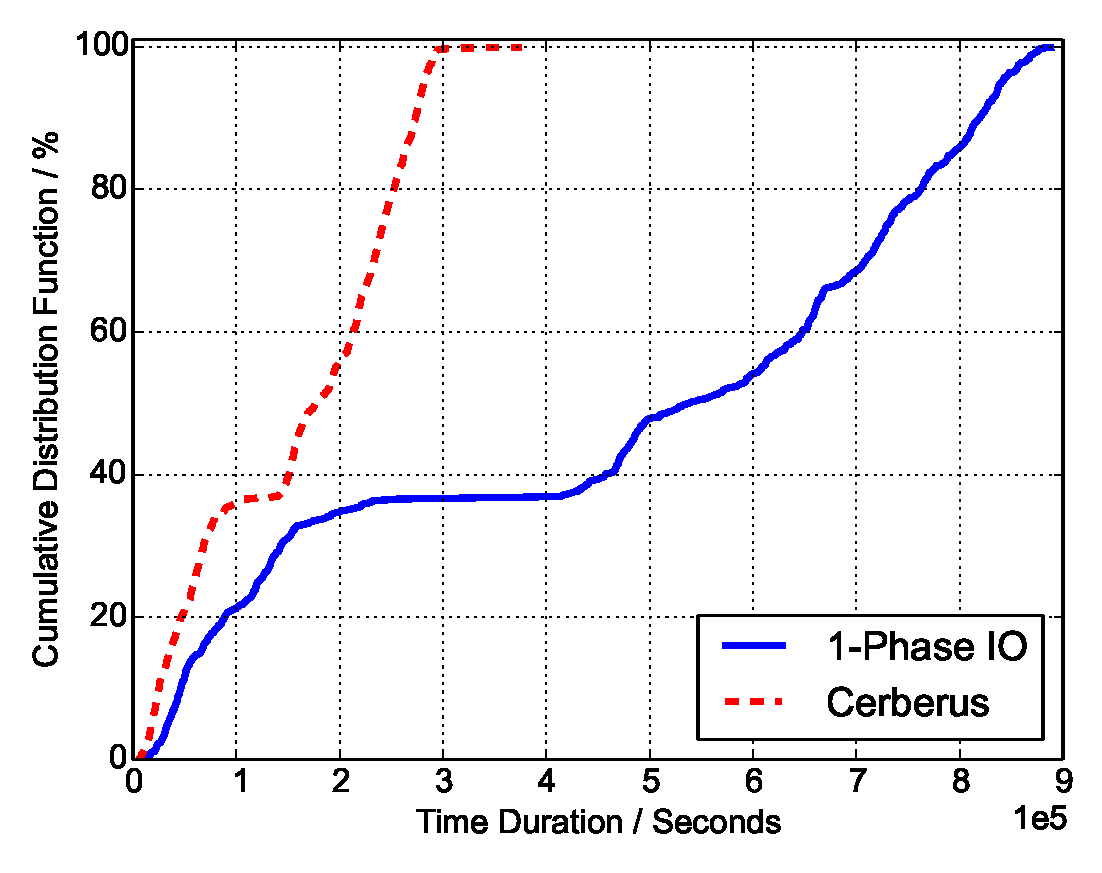
\includegraphics[width=2.2in]{IOvsBBFigures/1000jobs_direct_vs_bb_response}
                \label{Fig:DirectIOvsBBResponse}
        }
        \subfloat[Job Aggregated Wait Time] {
                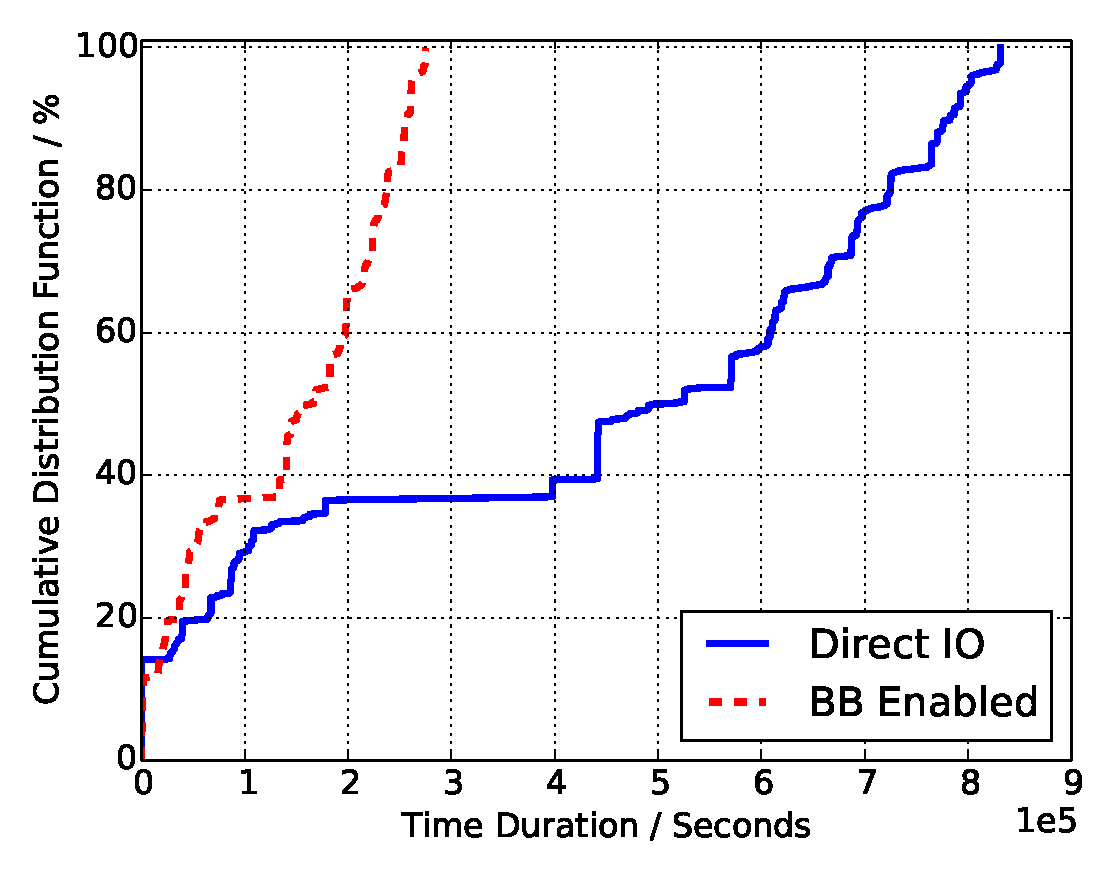
\includegraphics[width=2.2in]{IOvsBBFigures/1000jobs_direct_vs_bb_wait}
                \label{Fig:DirectIOvsBBWait}
        }
        \subfloat[System Throughput] {
                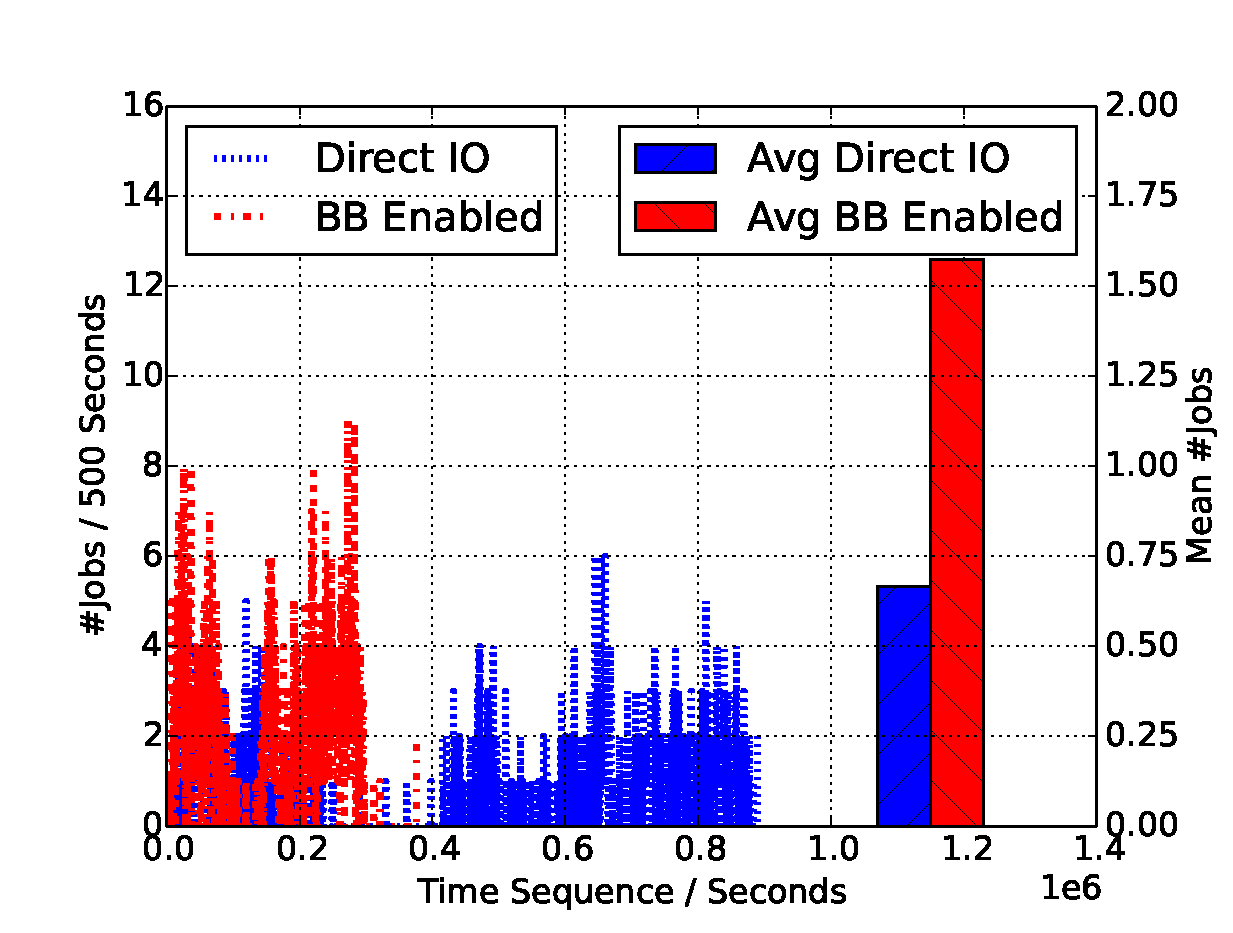
\includegraphics[width=2.5in]{IOvsBBFigures/1000jobs_direct_vs_bb_throughput}
                \label{Fig:DirectIOvsBBThroughput}
        }
        \caption{Utilizing Burst Buffer v.s. Direct IO}
        \label{Fig:DirectIOPerformance}
\end{figure*}

%\begin{figure}[!t]
        %\centering
        %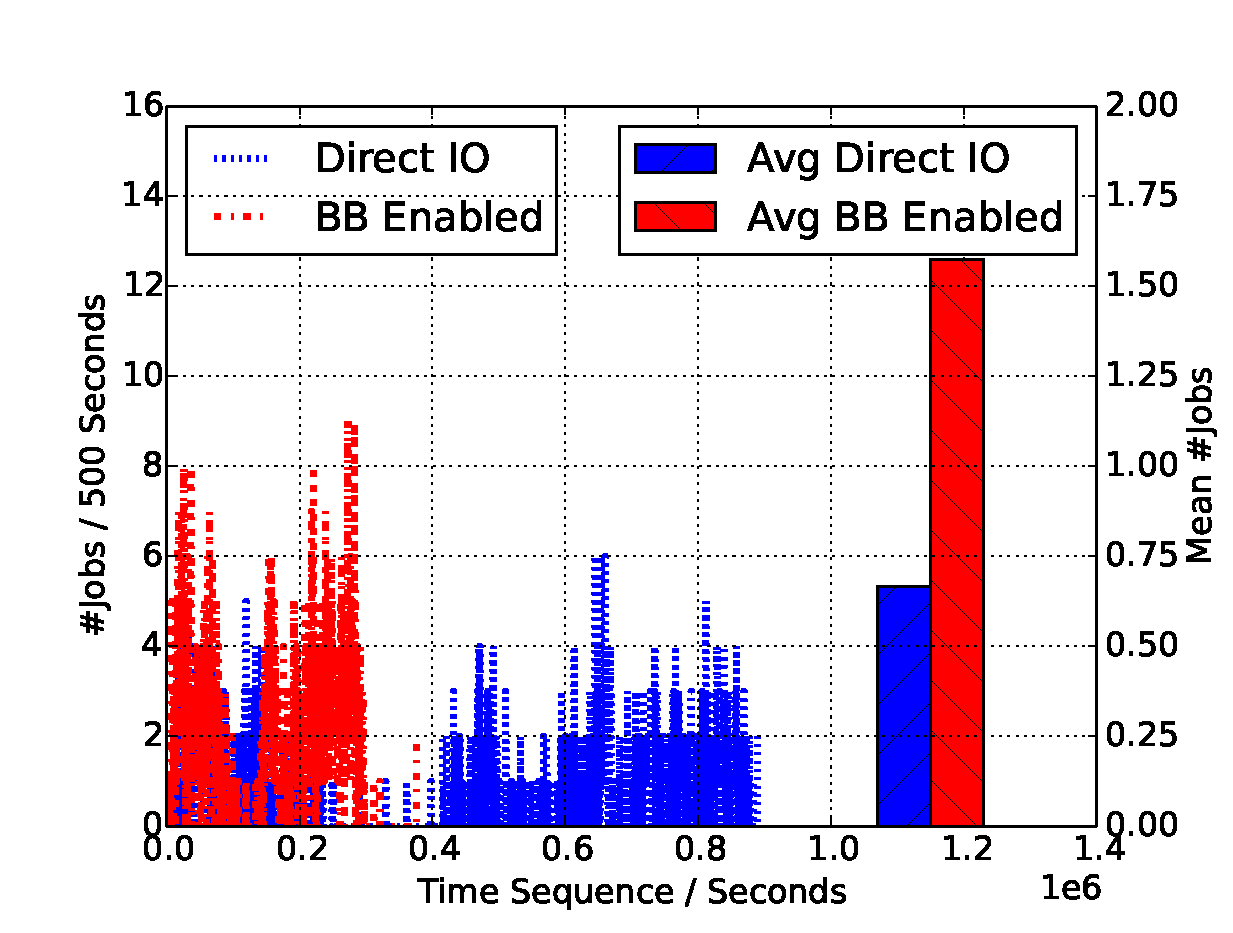
\includegraphics[width=3.2in]{IOvsBBFigures/1000jobs_direct_vs_bb_throughput}
        %\caption{System Throughput, IO Node Only vs. Burst Buffer System}
        %\label{Fig:DirectIOvsBBThroughput}
%\end{figure}


\subsection{Three-Phase Model v.s. One-Phase Model}
We validate our three-phase model by answering the question \textbf{Q2}.
Simulation results demonstrate that the job performance is improved 
when the scheduler makes scheduling decision in each phase separately.
Therefore, users are encouraged to provide detailed burst buffer demands in each phase for their jobs.

% In Figure~\ref{Fig:3Pvs1PResponse}, we plot 3 different scheduling results by 3 FCFS scheduler.
% \begin{itemize}
%         \item \textbf{1-Phase BB}: Jobs are modeled as just 1 phase.
%                 Users just provide general burst buffer demand throughout
%                 entire application lifetime.
%         \item \textbf{1D Cerberus}: In this case Cerberus only knows
%                 the overall burst buffer demand.
%         \item \textbf{Cerberus}: Users kindly provided all the burst buffer
%                 demand in all 3 phases.
%                 %the same as Cerberus in section~\ref{Sec:Sim:DirectIOvsBB}
% \end{itemize}
% We simulate the 3 cases with the same generated random data volume sequence.
% We assume the overall burst buffer demand in 1-phase BB and 1D Cerberus is
% $\max \{data\_in, data\_out, data\_run\}$.
% Notice that 1-phase BB scheduler must subject to burst buffer capacity constraint.
% %For 1-phase-modeled jobs, scheduler will make decision
% %based on $\max \{data\_in, data\_out, data\_run\}$
% %since we assume user will only tell the upper bound of its application's demand.
% %However, in simulation, we use the generated data amount as the same as 3-modeled jobs.
% %Response time of system without burst buffer devices are also plotted for comparison.

%========XY========================
In Figure~\ref{Fig:3Pvs1PResponse}, the scheduling results based on three models
are presented:
\begin{itemize}
        \item \textbf{1-Phase-1D}: Jobs are submitted with the total burst buffer demand,
        but their lifetime are not divided into three phases. 
	Instead, the scheduler makes scheduling decision only once for each job.

        \item \textbf{3-Phase-1D}: Jobs are submitted with the total burst buffer demand,
        their lifetime are divided into three phases as discussed in Section~\ref{Sec:Model}.
        
        \item \textbf{3-Phase-3D}: Jobs are submitted with the detailed burst buffer demand for each phase.
                %the same as Cerberus in section~\ref{Sec:Sim:DirectIOvsBB}
\end{itemize}
We simulate three cases with one set of randomly generated data volume sequences.
We assume the overall burst buffer demand in 1-Phase-1D and 3-Phase-1D is
$\max \{data\_in, data\_out, data\_run\}$.
Notice that 1-phase BB scheduler must subject to the burst buffer capacity constraint.
Cerberus is responsible for scheduling jobs in 3-Phase-1D and 3-Phase-3D model.
The scheduling policy used in this experiment is first-come first-serve.

% 
% %Unsurprisingly, jobs' response time is improving as long as they could utilizing burst buffer.
% When comparing scheduling results of 1-Phase BB and 1D Cerberus,
% both of which only have rough data information of application,
% more than 60\% of the 3-phase-modeled jobs finish faster than 1-phase-modeled jobs.
% The longest 3-phase-modeled job takes 418,927 seconds to finish
% while the slowest 1-phase-modeled job needs about 492,591 seconds to finish.
% The improvement is about 14.95\% for the worst case.
% The reason of such improvement is as follows.
% For the 1-phase-modeled jobs, burst buffer nodes will be exclusively
% taken by scheduled jobs throughout their lifetime.
% In contrast, Cerberus will reclaim burst buffer multiple times;
% it also releases burst buffer nodes and CPU resources as soon as possible.
% This gives Cerberus more opportunity to schedule the system resources.
% At last, when comparing the case of Cerberus with 1D Cerberus,
% we find another advantage of our 3-phase model.
% If benign users can provide finer-grain information of data/IO demand,
% Cerberus can programme each queue separately and get better scheduling result.
% In our simulation,
% since Cerberus knows more about application's demand in different phases,
% the worst absolute response time is less than 379,026 seconds.
% This is 10.24\% improvement to 3-phase-modeled jobs
% when Cerberus only knows the upper bound of data demand,
% 23.66\% better than the slowest 1-phase-modeled job.
% In average case, \textit{more than 80\% of the jobs 
% scheduled by Cerberus finish earlier than 1-phase-modeled jobs.}
% Meanwhile, \textit{more than 60\% of the jobs takes less time if user 
% specifies data usage demand at each phase to Cerberus, e.g. Cerberus vs. 3-Phase-1D.}


%==============XY===============
When comparing the scheduling results of 1-Phase-1D and 3-Phase-1D,
both of which only have the overall burst buffer demand of each job,
more than 60\% of the three-phase-modeled jobs finish faster than the 1-phase-modeled jobs.
The slowest three-phase-modeled job takes 418,927 seconds to finish,
while the slowest 1-phase-modeled job takes about 492,591 seconds to finish.
The improvement is about 14.95\% in the worst case scenario.
Here is the explanation: For the 1-phase-modeled jobs, the burst buffer nodes will be exclusively
taken by the scheduled jobs throughout their lifetime. In contrast, Cerberus reclaims the burst buffer multiple times;
It also releases the burst buffer nodes and the CPU resources at the earliest possible time, which allows Cerberus to schedule more system resources.
%Finally, when comparing the cases of 3-Phase-3D with 3-Phase-1D, we find another advantage of our 3-phase model.
In addition, if benign users can provide fine-grain information of data/IO demands,
Cerberus can program each queue separately and achieve better scheduling result.
For the 3-Phase-3D model, Cerberus knows each job's demand during the different phases,
the worst absolute response time is less than 379,026 seconds.
This is about 10.24\% improvement to three-phase-modeled jobs.
When Cerberus only knows the upper bound of data demand,
it is 23.66\% better than the slowest 1-phase-modeled job.
In average, \textit{more than 80\% of the three-phase-modeled jobs
finish earlier than 1-phase-modeled jobs.}
Meanwhile, \textit{more than 60\% of the jobs take less time if user
specifies data usage demand at each phase, e.g., 3-Phase-3D vs. 3-Phase-1D.}



% We can reason about why Cerberus's scheduling result is better than
% naively integrating batch scheduler with burst buffer constraint
% by looking at the detailed waiting time.
% Figure~\ref{Fig:3Pvs1PWaitRun} shows the time job spend in running queue.
% There are 3 queues in Cerberus;
% correspondingly we have 3 kinds of waiting for jobs in Cerberus.
% %Figure~\ref{Fig:3Pvs1PWaitIn} shows the time job spend in inputing queue,
% %Figure~\ref{Fig:3Pvs1PWaitOut} the time job spend in outputing queue.
% For 1-phase-modeled jobs, there is just one queue;
% therefore the waiting time in Figure~\ref{Fig:3Pvs1PWaitRun} is the total waiting time.
% We see that jobs did not spend much time in either input queue $Q_I$ or output queue.
% The upper bounds of time spent in input queue are
% 2500 seconds for 1D Cerberus and Cerberus respectively.
% This is because input data is very small (tens of GB level)
% comparing to checkpointing data and application output (tens of TB level).
% In contrast, in worst case job scheduled by 1-Phase BB needs to wait for 443,203 seconds,
% because scheduler makes one-time decision on the basis of demand of
% both computer node and maximum burst buffer.
% %the upper bounds of time spent in output queue $Q_O$ are
% %less than 5\% of the total waiting time of 1-phase-scheduler case
% %for both 3-phases cases.
% As for the time waiting for running, more than 60\% of the jobs scheduled by
% 1D Cerberus and Cerberus are better than 1-phase-modeled jobs.
% The difference of waiting time results in the different
% response performance.


We now investigate the detailed waiting time to understand why the scheduling results in Cerberus
are better than the naive integration of the batch scheduler with the burst buffer constraints.
Figure~\ref{Fig:3Pvs1PWaitRun} shows the waiting running time, how long a job spent in the running queue.
There are three queues in Cerberus;
Correspondingly jobs in Cerberus have three kinds of waiting time: waiting input, waiting running, and waiting output time.
%Figure~\ref{Fig:3Pvs1PWaitIn} shows the time job spend in inputing queue,
%Figure~\ref{Fig:3Pvs1PWaitOut} the time job spend in outputing queue.
For 1-phase-modeled jobs, there is just one queue;
Therefore, the waiting time in Figure~\ref{Fig:3Pvs1PWaitRun} is the total waiting time.
We observe that (not shown in Figure~\ref{Fig:3Pvs1PWaitRun}) the jobs did not
take much time either in the input queue $Q_I$ nor in the output queue.
The upper bounds of time spent in the input queue, e.g. waiting time in $Q_I$, are 
2,500 seconds for both 3-Phase-1D and 3-Phase-3D modeled jobs.
This is because that the input data are very small (e.g., tens of GB)
compared to the checkpointing data and the application output (e.g., tens of TB).
In contrast, in the worst case of 1-Phase-1D, the job waiting time is 443,203 seconds,
because the scheduler makes a one-time decision based on the demand of the computer node and the maximum burst buffer.
%the upper bounds of time spent in output queue $Q_O$ are
%less than 5\% of the total waiting time of 1-phase-scheduler case
%for both 3-phases cases.
As for the time waiting for running, more than 60\% of the 3-Phase-1D and 3-Phase-3D modeled jobs are scheduled,
which is much better than the 1-phase-model.
The differences of the waiting time lead to the difference in response performance.


% Figure~\ref{Fig:3Pvs1PThroughput} describes system throughput of these three different scenarios.
% It helps us examine the performance of the scheduling in time sequence.
% For 1-phase-modeled job, we can see an obvious `throughput gap'
% from 150,000 second to 200,000 second approximately,
% similar for the case of 1D Cerberus, throughput also starts provocatively,
% Cerberus' runs counter to both previous cases.
% Even though there is a throughput trough between 100,000 to 150,000 seconds,
% Cerberus manages to make the system having high throughput at the beginning and
% later (from 150,000 to 300,000 seconds).
% \textit{In average, the throughput of Cerberus is 1.575 jobs / 500 seconds.}
% It is 11.39\% of the 1-Phase BB case (1.414 jobs / 500 seconds) and
% 31.03\% higher than the 1D Cerberus case (1.202 jobs / 500 seconds).
% We believe this validates the indispensable 3 phase job model and
% the necessity that user provides data capacity demand for each phase.

Figure~\ref{Fig:3Pvs1PThroughput} describes the system throughputs of the three different job models.
It helps us to examine the scheduling performance in a time sequence.
For 1-Phase-1D modeled job, we can see an obvious `throughput gap'
from 150,000 seconds to 200,000 seconds approximately.
The case of 3-Phase-1D Cerberus is similar.
3-Phase-3D runs counter to both previous cases.
Even though there is a throughput between 100,000 to 150,000 seconds,
the 3-Phase-3D model manages to make the system having a high throughput at the beginning and
later changes from 150,000 to 300,000 seconds.
\textit{In average, the throughput of the 3-Phase-3D model is 1.575 jobs / 500 seconds.}
It is 11.39\% higher than the 3-Phase-1D case (1.414 jobs / 500 seconds) and
23.68\% higher than the 1-Phase-1D case (1.202 jobs / 500 seconds).
We believe that the results validate the indispensable 3 phase job model and
justifies the necessity that a user needs to provide data capacity demand for each phase.



\begin{figure*}[htp]
        \centering
        \subfloat[Job Response Time] {
                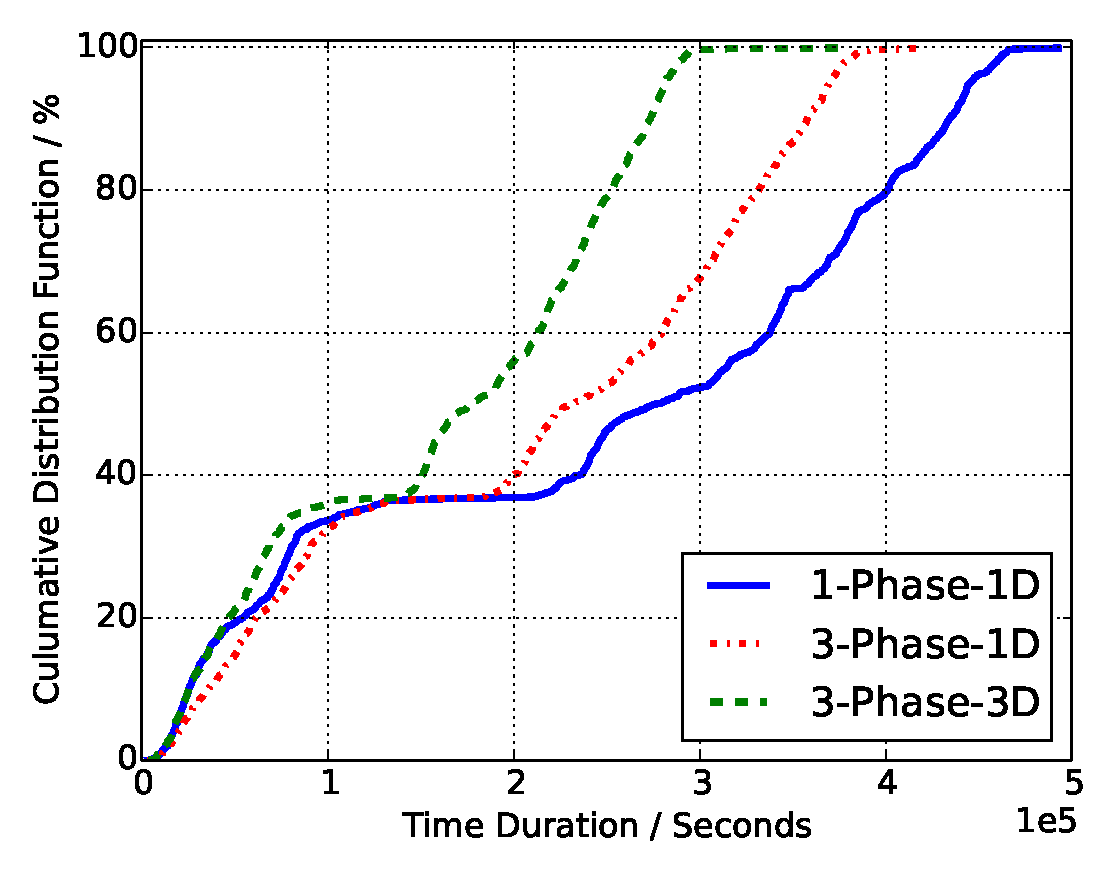
\includegraphics[width=2.2in]{3Pvs1PFigures/1000jobs_3p_vs_1p_response}
                \label{Fig:3Pvs1PResponse}
        }
        %\subfloat[Job Wait Time] {
                %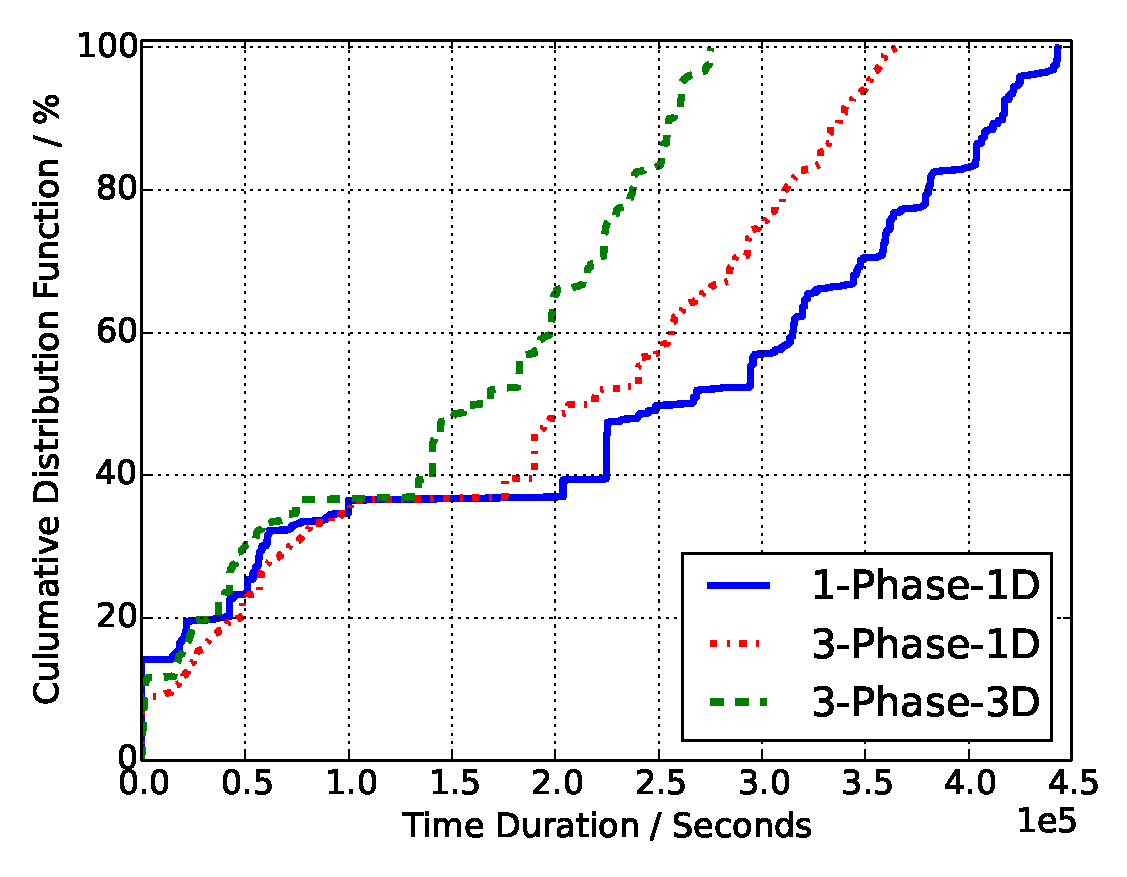
\includegraphics[width=3.2in]{3Pvs1PFigures/1000jobs_3p_vs_1p_wait}
                %\label{Fig:3Pvs1PWait}
        %}
        %\subfloat[Job Wait Input Time] {
                %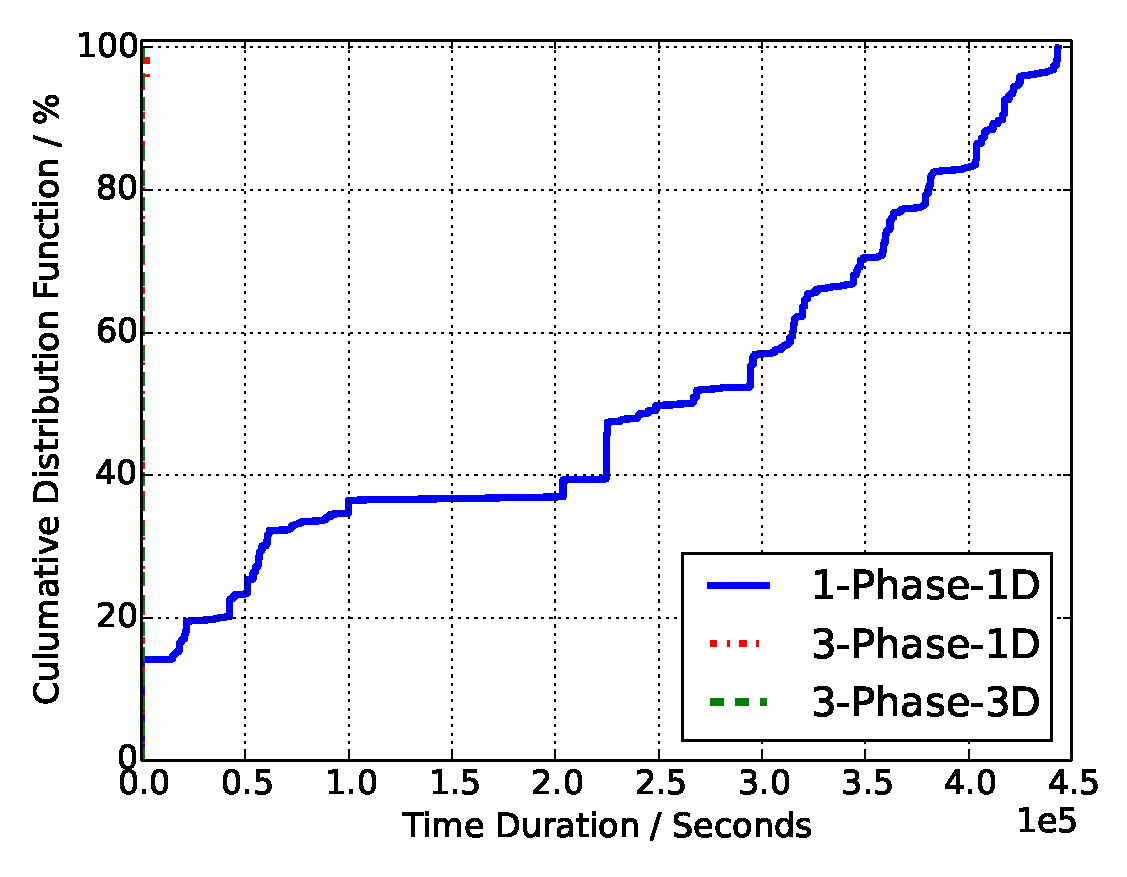
\includegraphics[width=2.3in]{3Pvs1PFigures/1000jobs_3p_vs_1p_wait_in}
                %\label{Fig:3Pvs1PWaitIn}
        %}
        %~
        \subfloat[Job Waiting Time in $Q_R$] {
                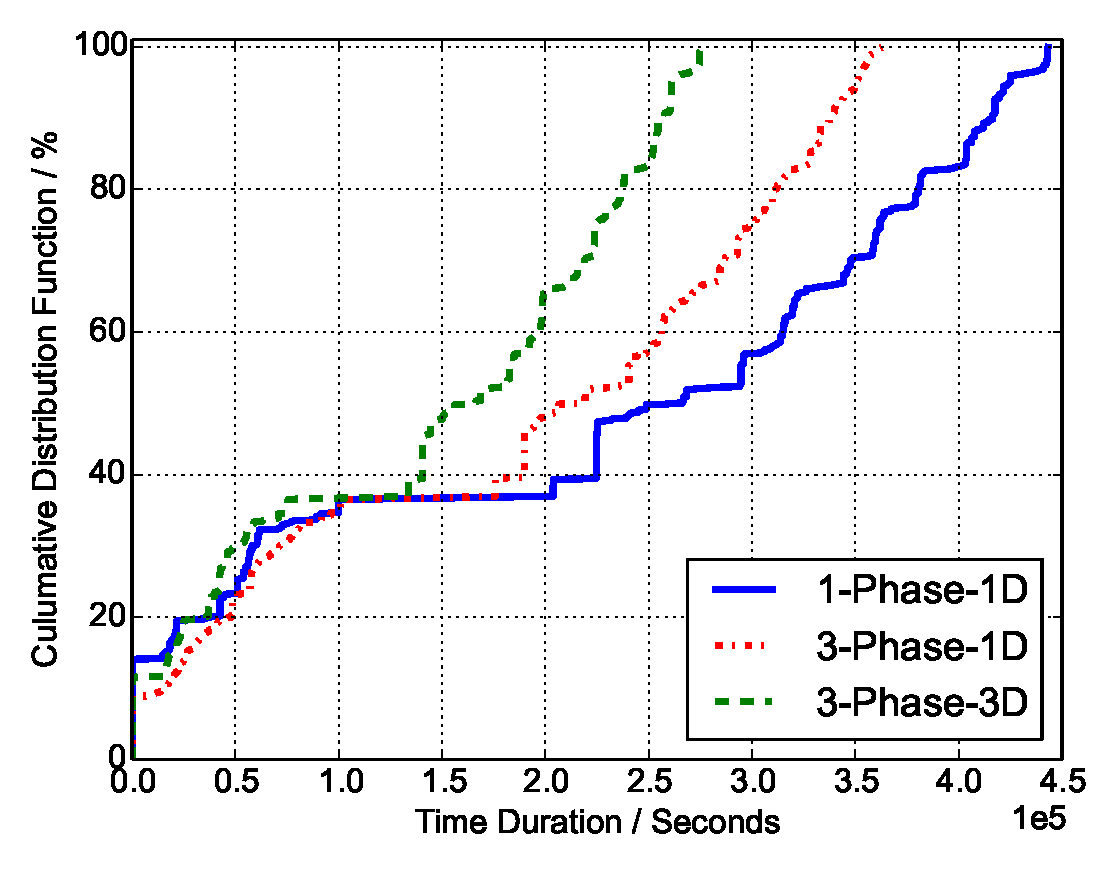
\includegraphics[width=2.2in]{3Pvs1PFigures/1000jobs_3p_vs_1p_wait_run}
                \label{Fig:3Pvs1PWaitRun}
        }
        \subfloat[System Throughput] {
                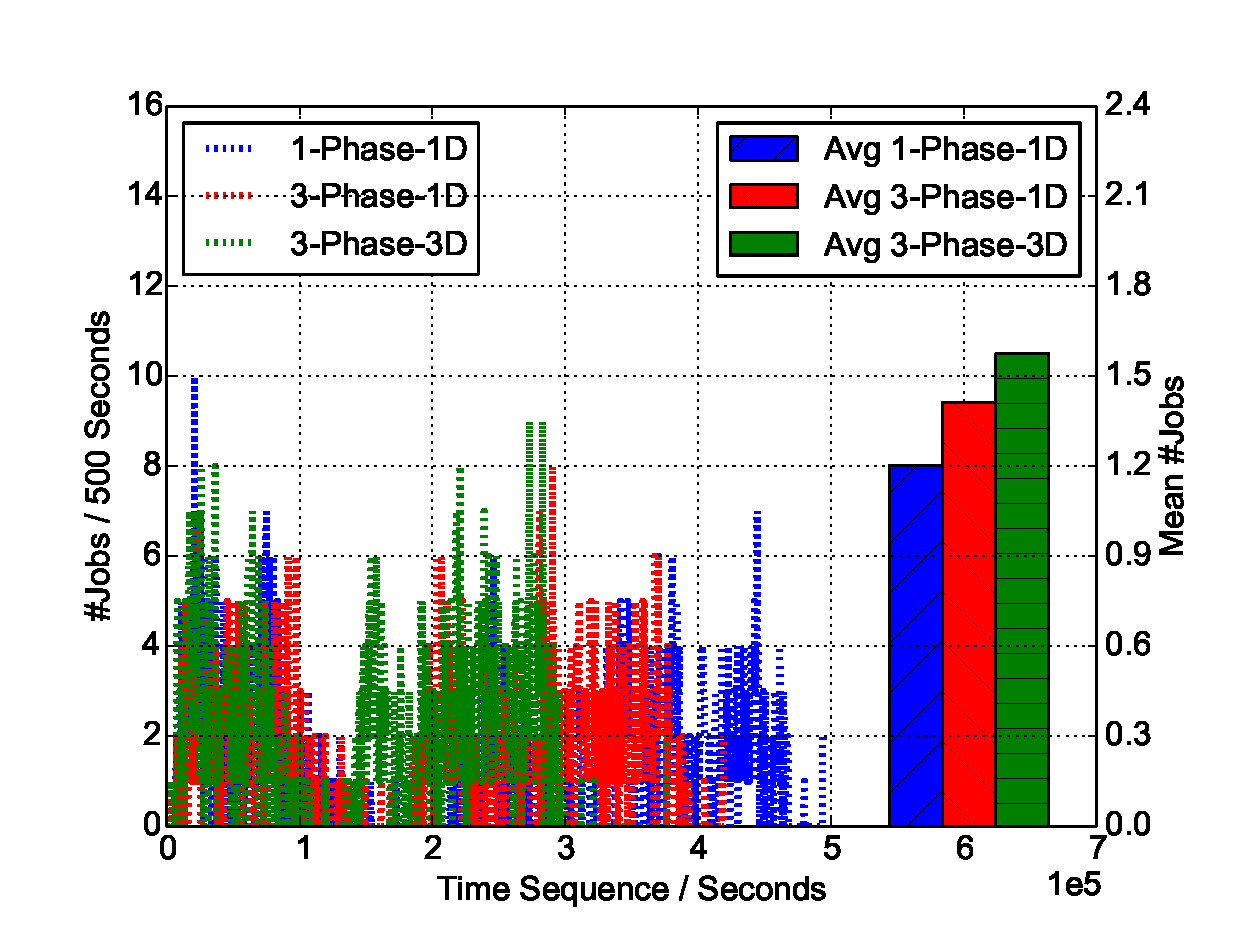
\includegraphics[width=2.5in]{3Pvs1PFigures/1000jobs_3p_vs_1p_throughput}
                \label{Fig:3Pvs1PThroughput}
        }
        \caption{Three-Phase Model vs. One-Phase Model}
        \label{Fig:3Pvs1PPerformance}
\end{figure*}

%\begin{figure}[!t]
        %\centering
        %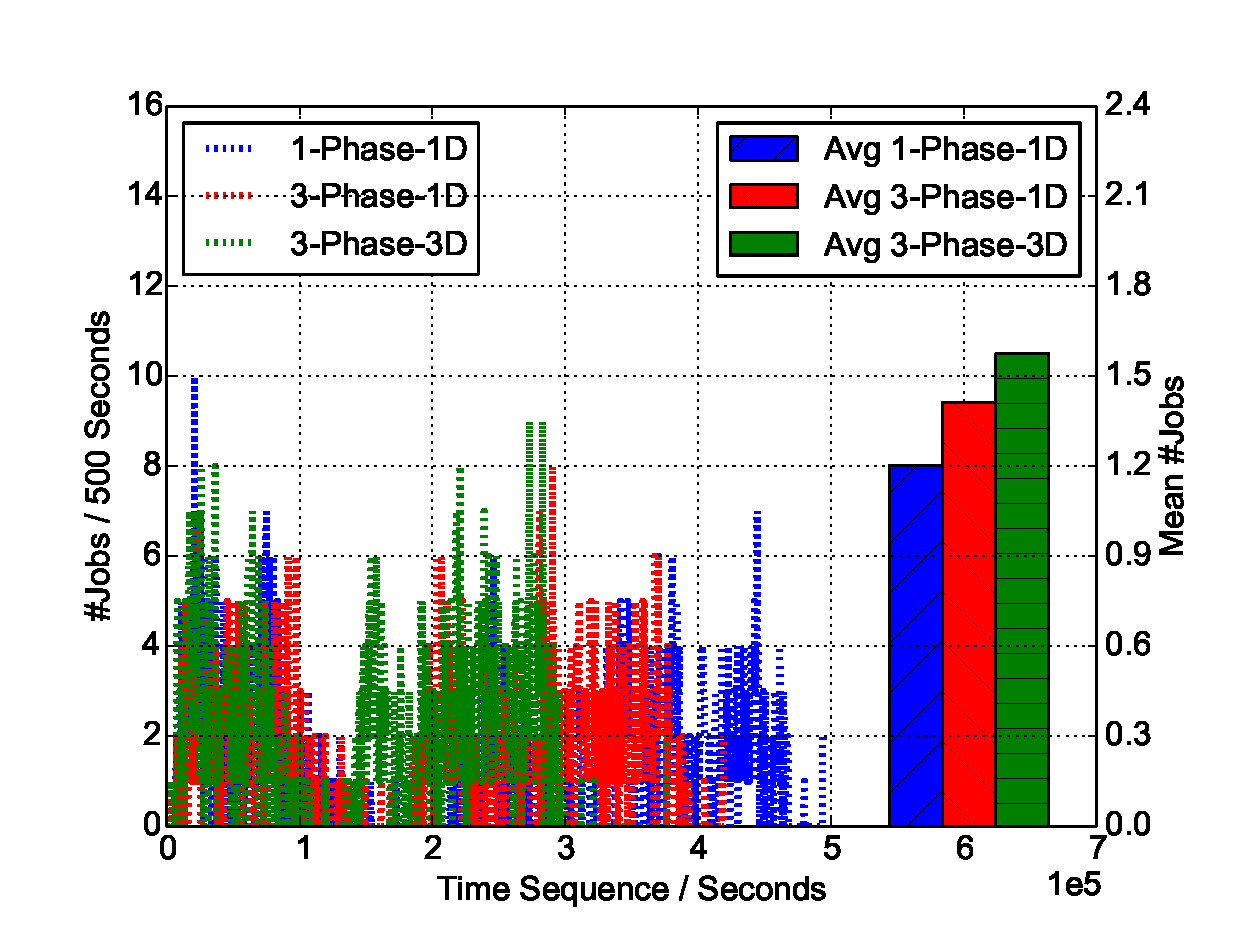
\includegraphics[width=3.2in]{3Pvs1PFigures/1000jobs_3p_vs_1p_throughput}
        %\caption{System Throughput, 1 Phase Model vs. 3 Phase Model}
        %\label{Fig:3Pvs1PThroughput}
%\end{figure}

\begin{figure*}[htp]
        \centering
        \subfloat[Job Response Time] {
                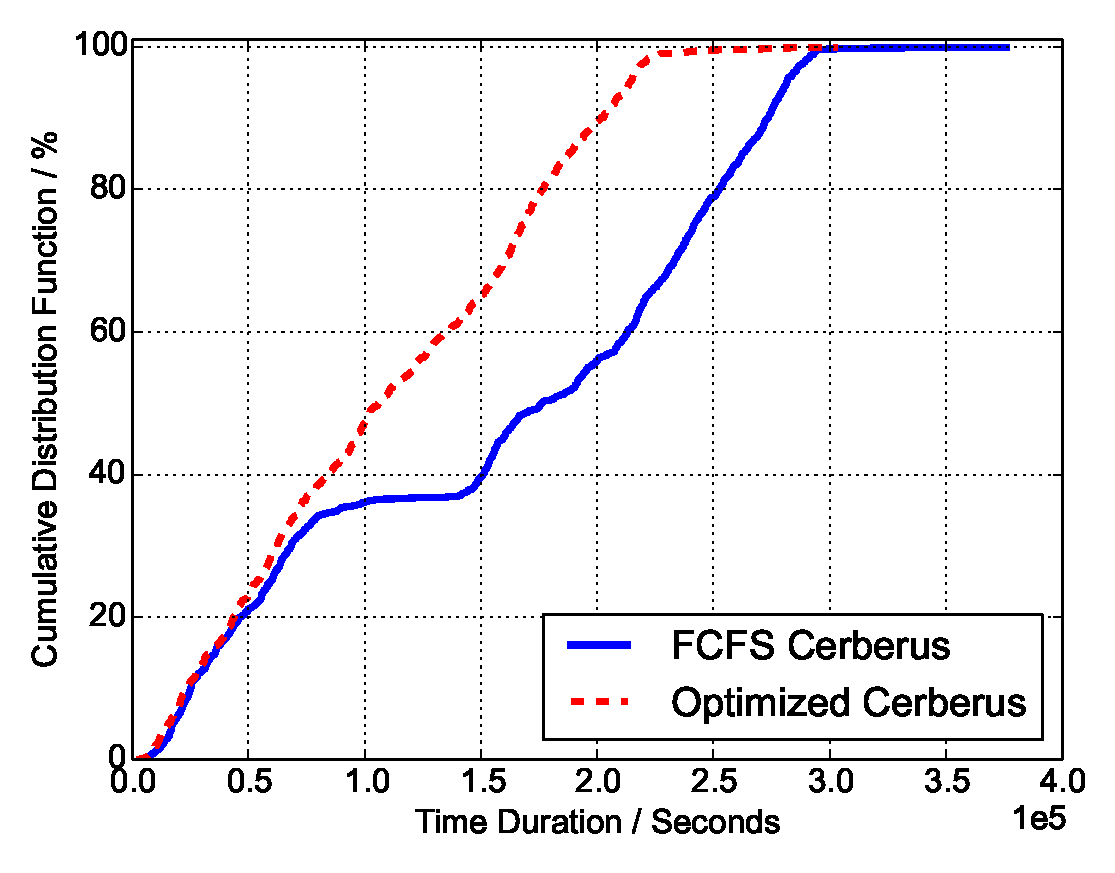
\includegraphics[width=2.2in]{DPvsFIFOFigures/1000jobs_dp_vs_fifo_response}
                \label{Fig:DPvsFIFOResponse}
        }
        \subfloat[Job Aggregated Waiting Time in $Q_R$] {
                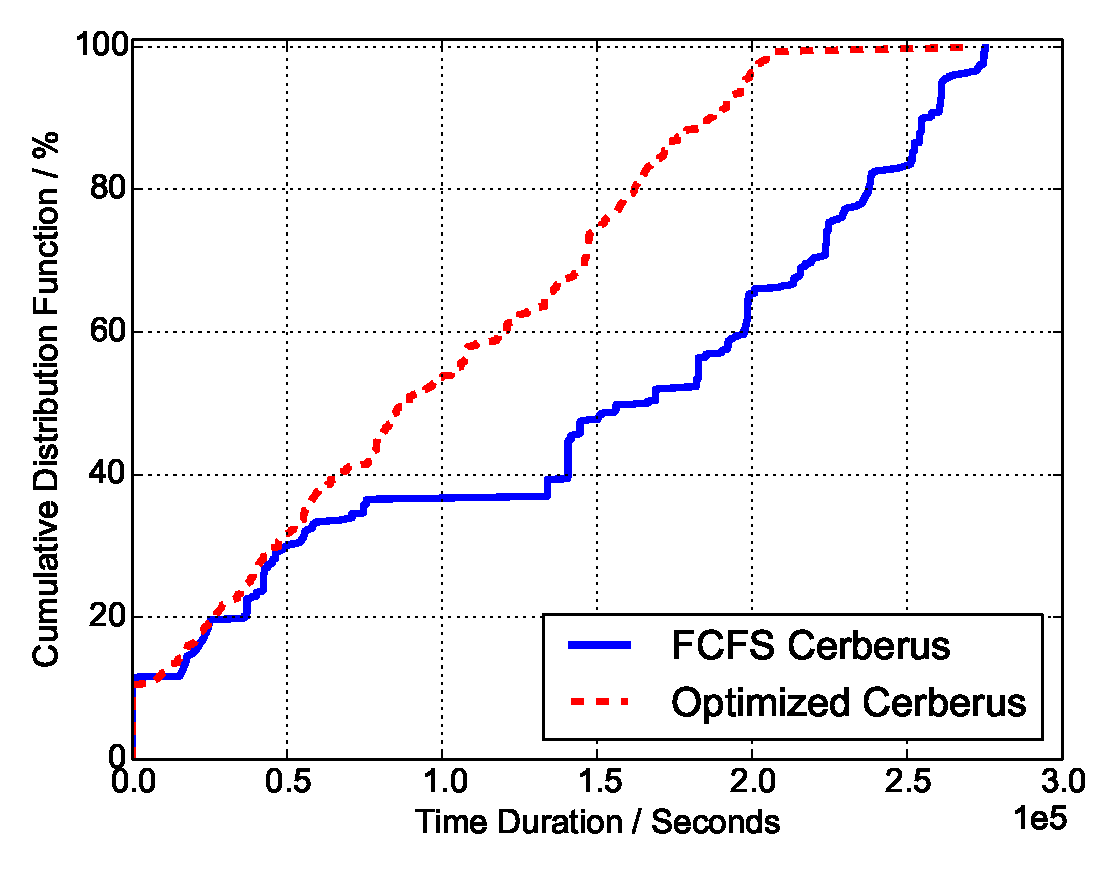
\includegraphics[width=2.2in]{DPvsFIFOFigures/1000jobs_dp_vs_fifo_wait_run}
                \label{Fig:DPvsFIFOWaitRun}
        }
        \subfloat[System Throughput] {
                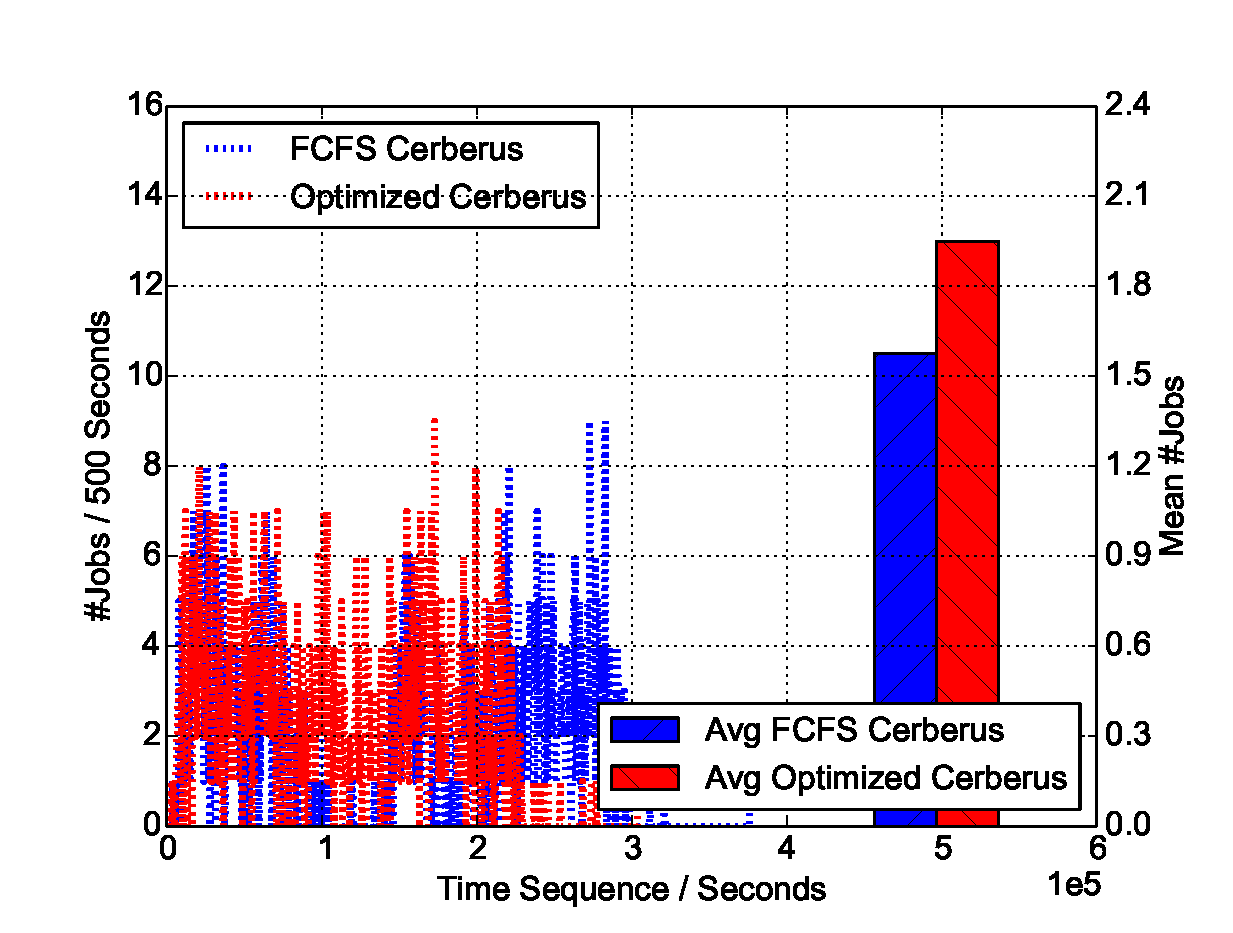
\includegraphics[width=2.5in]{DPvsFIFOFigures/1000jobs_dp_vs_fifo_throughput}
                \label{Fig:DPvsFIFOThroughput}
        }
        \caption{Cerberus v.s. FCFS}
        \label{Fig:DPvsFIFOPerformance}
\end{figure*}

%\begin{figure}[!t]
        %\centering
        %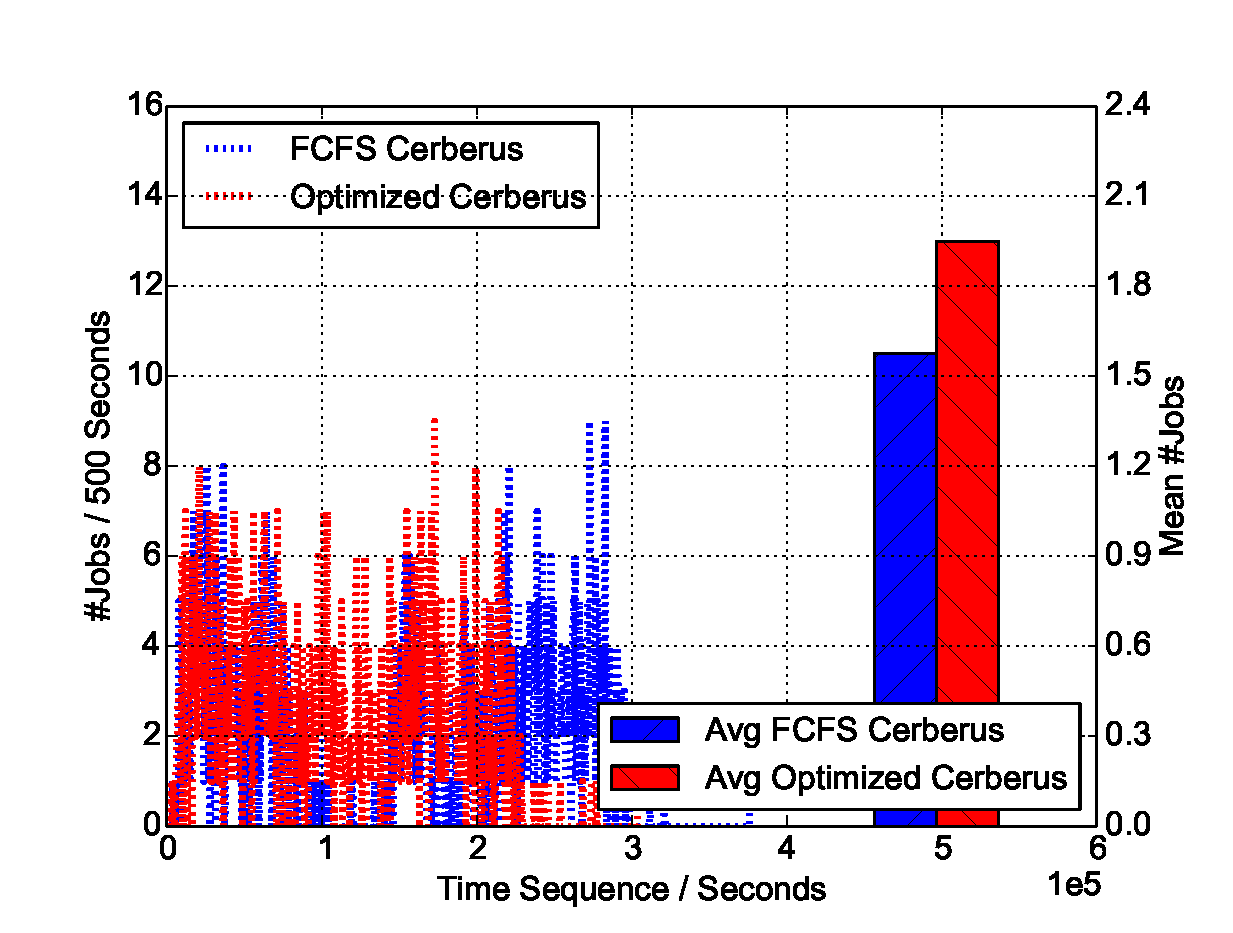
\includegraphics[width=3.2in]{DPvsFIFOFigures/1000jobs_dp_vs_fifo_throughput}
        %\caption{System Throughput, Optimized Cerberus vs. FCFS Cerberus}
        %\label{Fig:DPvsFIFOThroughput}
%\end{figure}

\subsection{Cerberus v.s. FCFS Three-Phase Scheduling}
%If we consider optimizing either burst buffer's data throughput or the parallelism across jobs,
%dynamic programming based job scheduler can further reduce jobs' wait time.
%We plot in Figure~\ref{Fig:DPvsFIFOResponse} the resulting response time of
%two versions of Cerberus:
%\begin{itemize}
%        \item \textbf{FCFS Cerberus} uses naive first come first serve policy.
%                Whoever at the front of queue are considered favorably.
%        \item \textbf{Optimized Cerberus} select these jobs in $Q_I$ and $Q_O$
%                such that volume of to be transferred data
%                is maximized by Recursion~\ref{Equ:MaxTransferDataRecursion}.
%                For jobs in $Q_R$, it chooses jobs according to the optimization solution
%                given by Equation~\ref{Equ:MaxProductRecursion}
%\end{itemize}
%As indicated by Figure~\ref{Fig:DPvsFIFOResponse}, response time of
%jobs scheduled by Optimized Cerberus is reduced.
%The most non-responsive job for Optimized Cerberus is job \#445,
%taking 303,523 seconds.
%In contrast, job \#445 takes 376,026 seconds to finish in FCFS Cerberus.
%This is 19.28\% slower than Optimized Cerberus.
%When we consider the overall response time of entire job set,
%we see more than \textit{80\% of the tasks response faster when we do optimization}.

%===========XY===============
In this section, we answer the question \textbf{Q3} by showing that
adopting optimization in each scheduling phase can bring further improvement,
compared with a naive first come first server (FCFS) three-phase scheduling design.
Specifically, in the stage-in and stage-out phases, Cerberus schedules the jobs in $Q_I$ and $Q_O$
according to the solution given by \equref{Equ:MaxTransferDataRecursion};
for jobs in $Q_R$, Cerberus makes the scheduling decisions
based on the solution given by \equref{Equ:MaxProductRecursion}. %Algorithm~\ref{Alg:MaxCPU}.
We denote these two scheduling designs
as \textbf{FCFS} and \textbf{Cerberus} respectively.

As indicated by Figure~\ref{Fig:DPvsFIFOResponse}, the job response time scheduled by Cerberus is reduced.
The most non-responsive job for Cerberus is job \#445, which takes 303,523 seconds to complete.
In contrast, job \#445 takes 376,026 seconds to finish in FCFS.
This is 19.28\% slower than the Cerberus.
When we consider the overall response time of the entire job set,
we observe that more than \textit{80\% of the jobs response faster when scheduled by Cerberus}.


The time duration that an application is waiting for running
is plotted in Figure~\ref{Fig:DPvsFIFOWaitRun}.
The tail of Cerberus shows that a couple of jobs
spend very long time in the running queue.
This is because: First the jobs are submitted at the early middle phase
(job \#435 waits for 268,322 seconds); Second, these jobs request a huge
amount of compute nodes (10240), but comparably less amount of burst buffer (7 TB for job \#435);
Third, there are jobs requesting a large number of cores but requesting
less running time and a larger amount of burst buffer.
For example, job \#434 requests 10,240 compute nodes but the expected running time
is only 3,600 seconds and it also requests 59 TB burst buffer.

As a result, Cerberus favors the jobs with less requesting time and larger burst buffer demand,
according to \equref{Equ:MaxProductRecursion}.
This is interesting because it is a potential flaw in the optimization-based policy:
Given that the users know the optimization objective of the scheduler,
it is possible for a user to cheat the scheduler with false demands.
%In other words, our optimization scheme, even though providing performance enhancement
%for the waiting time of 70\% jobs, is not strategy-proofness\cite{Ghodsi:NSDI:2011}


We can see the system throughputs under different scheduling objectives in Figure~\ref{Fig:DPvsFIFOThroughput} .
When scheduled by Cerberus, it takes 303,940 seconds to finish the workload,
while FCFS takes 376,443 seconds to complete the same workload.
The worst case completion time improvement of Cerberus over FCFS is 19.26\%.
When we look at the time sequence of throughput,
we found that the peak value 9 jobs / 500 seconds can be finished when scheduled by Cerberus.
The peak throughput of the FCFS is also 9 jobs / 500 seconds.
The mean throughputs of these three scheduling methods are plotted in Figure~\ref{Fig:DPvsFIFOThroughput}.
Compared with the FCFS, \textit{the Cerberus achieves about 23.87\% higher average throughput}
(1.951 jobs / 500 seconds).


%Table~\ref{Tab:OptimizationTime} demonstrate that 
% % Memoization technique helps optimized Cerberus be able to schedule jobs online,
% % though solving the optimization problem is theoretically NP-hard.
% % For Optimized Cerberus, it solved about 8400 Problem~\ref{Equ:MaxTransferData} and
% % Problem~\ref{Equ:MaxProduct} when scheduling all the jobs in workload,
% % taking less than 370 seconds.
% % The time overhead of solving each optimization is about 0.04 seconds per time.

%\begin{table}[!t] 
        %\renewcommand{\arraystretch}{1.3}
        %\caption{Time Consumption in Dynamic Programming}
        %\label{Tab:OptimizationTime}
        %\centering
        %\begin{tabular}{l|c}
                %\hline
                %Optimization Policy Used & Optimized Cerberus\\
                %\hline
                %\hline
                %Simulation Run Time / seconds & 375.55\\
                %Optimization Run Time / seconds & 364.62\\
                %Total Number of Optimizations & 8406\\
                %\hline
        %\end{tabular}
%\end{table}

Memorization technique helps the Optimized Cerberus to perform online job scheduling,
though solving the optimization problem is theoretically NP-hard.
In our simulation, it takes about 0.04 second in average for the Cerberus to make a scheduling decision.


